\chapter{Design}

In this chapter, the process of deciding upon and making the design of the Physical interface (music educational tool), will be explained. The design will be based on the formulated design requirements (see \autoref{sec:DRequirements}), as well as the common design principles of Gestalt \cite{gestalt}, the SOTA ( \autoref{sec:sota}) and knowledge gained from the workshop at Sankt Annæ (see \autoref{sec:workshop}). 


\section{Intial design}
The design of the physical interface was, with the design requirements, not specified to the extend, that a specific concept for the design was obvious. The design could instead be taken in broad variety of directions, and still live up to the requirements. As so, the design of the physical interface has been though lots of different concepts and iterations. 

\subsection {Workshop prototypes - The pre-initial designs}

During the analysis, a need for educational tools that were built with collaboration in mind, was discovered (see \autoref{sec:problemArea}). Based on that, multiple low fidelity initial concepts were created and brought to Sankt Annæ for an ideation workshop. As mentioned in \autoref{sec:problemArea}, the prototypes at this point were used to discuss and discover new concepts and elements, which could be utilized in the final design. The findings from this workshop did not necessarily lead to new requirements, but instead served as pointers to which direction the design could be taken. For example, the tool could make use of movement, which might conflict with or move the focus away from the learning aspect, and (in such a case) should be avoided. In another case, movement might serve to enhance the learning outcome (see \autoref{AnalysisMovement}), and should therefore be strived for. This however depends on the individual concept, and each find from the workshop should therefore be discussed in relation to each design idea.\\\\

In order to evaluate upon many different elements and ways of collaborating and learning music, the aim of the concepts behind the prototypes, was to differ significantly from one another. Both the topic of the material to be learned, and the way to work with this, was therefore different for each of the concepts. Each concept will be briefly described in the following figure \todo{make figure}.
\todo{lav "collage" med ideer og giv kort beskrivelse af concept ( ryste klods,joystic band,chord master felx ,frugt løkker,quizz game, sequencer square..   A physical version of \textit{Garage Band}. }

\begin{figure}[H]
	\centering
	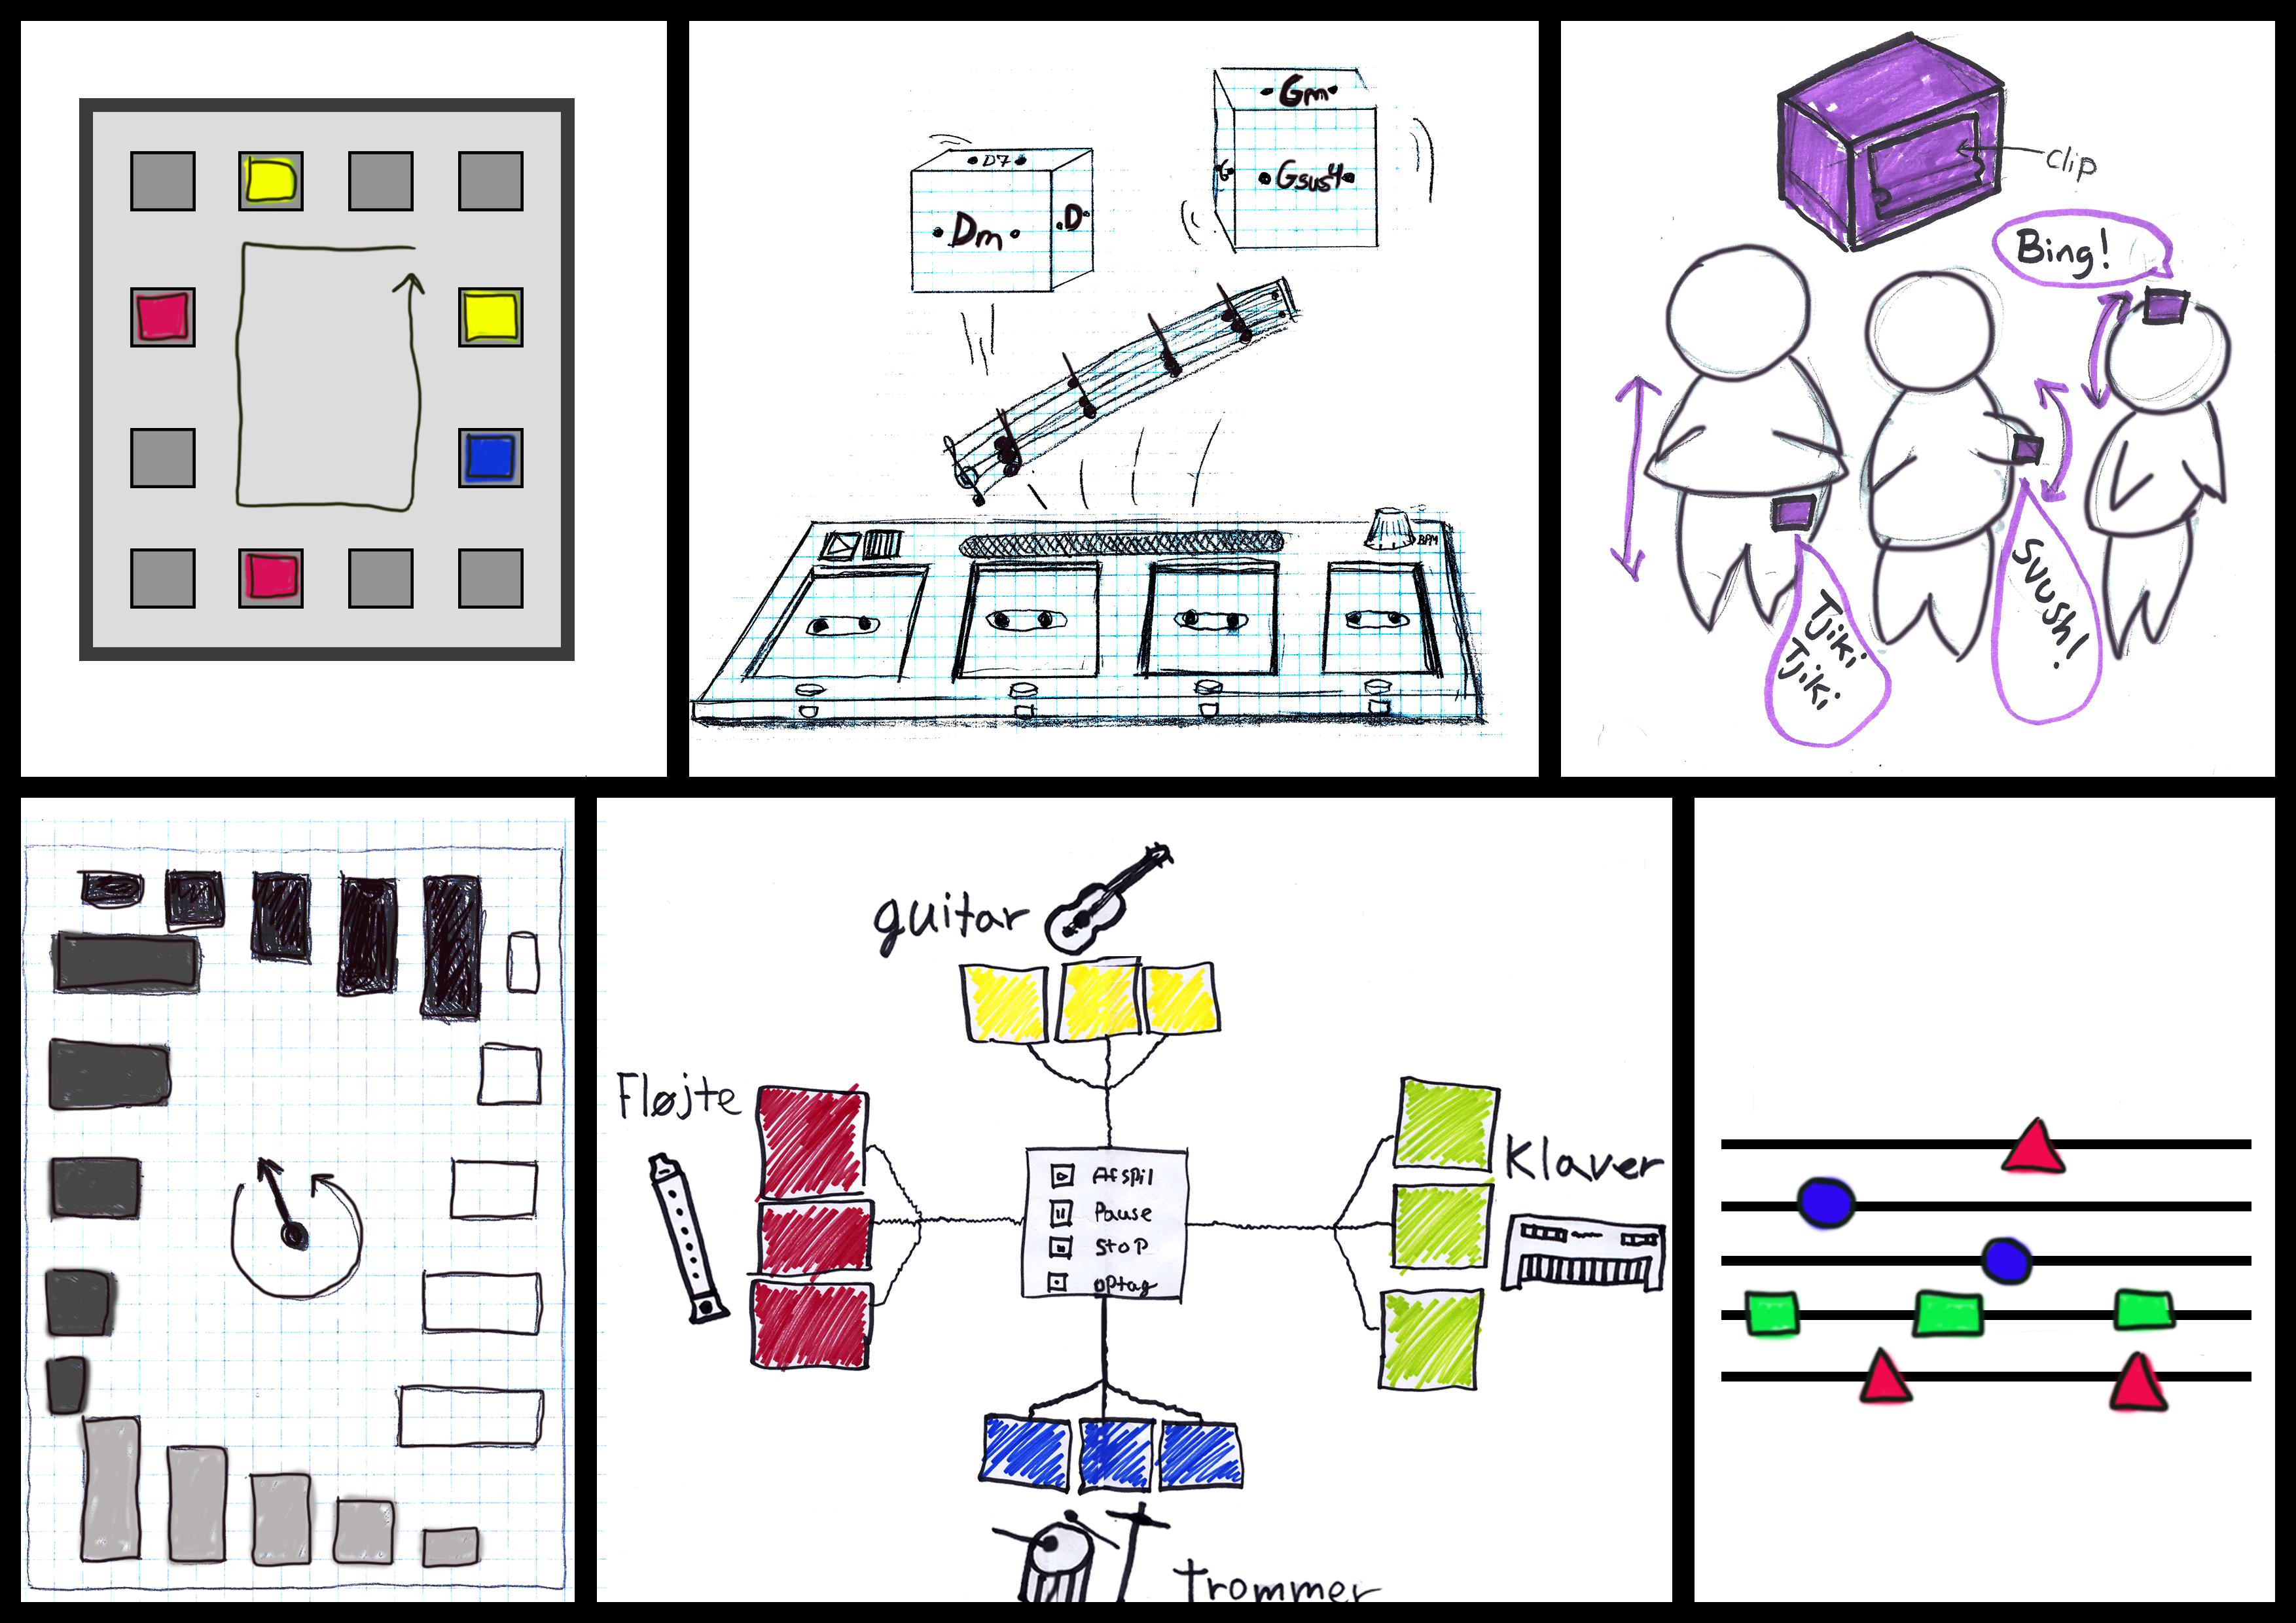
\includegraphics[width=0.9\linewidth]{figure/Design/workshopPrototypesDone} 
	\caption{Seen is the 6 design concepts which were precented at the workshop at Sankt Annæ. Top left: a device that loops though entries(squares), and plays sounds if a box is placed on the entry point. Top middle: an ear training tool, where boxes labeled with tone names, should be orientated to display the heard tone. Top right: Wearables which produces individual sounds when shaken. can be used to create and perform music - alike STOMP. Bottom left: Board of a quiz game with music theory questions. Bottom middle: A set of joysticks to play instruments in a "band setting". Bottom right: A physical version of \textit{Garage Band}\cite{Garageband}.}
	\label{fig:workshopPrototypes}
\end{figure}
\todo{erstat med "collage" med ideer og giv kort beskrivelse af concept ( ryste klods,joystic band,chord master felx ,frugt løkker,quizz game, sequencer square..1. quiz game with music theory questions  2. Wearables which produces individual sounds when shaken. can be used to create and perform music - alike STOMP 3. a set of joysticks to play instruments in a "band setting". 4. A physical version of \textit{Garage Band}. 5. loops though entries, and plays sounds if a box is placed on the entry point. 6. Ear training tool, where boxes labeled with tone names, should be orientated to display the heard tone.}



\subsection{From workshop and requirements - the Crawford slip method}
To evaluate upon the workshop prototype concepts, in relation to the design requirements formulated and the knowledge gained from the workshop, a custom version of the Crawford slip method was used (\autoref{secc:designMethod}) \todo{fix label then method is done!}. By doing this, a list of suggestions to how elements could be used, and should not be used, was made and used as inspiration for other concept ideas. A sample of the list can be seen in figure \autoref{fig:snippetOfList}. The full list can be seen in the appendix \autoref{CrawfordSlipList}.  

\begin{figure}[H]
	\centering
	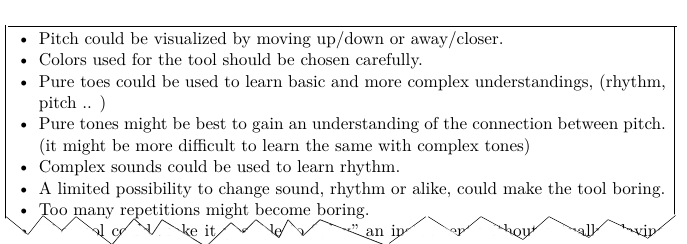
\includegraphics[width=0.7\linewidth]{figure/Design/snippetOfList} 
	\caption{Seen is a small section of the design suggestion list, based on the custom version of the Crawford slip method.}
	\label{fig:snippetOfList}
\end{figure}


With the project group divided into two groups of three persons, two design concept was created (one for each group), with inspiration form this list. These two concepts, was then presented between the two groups, and discussed.  

\subsubsection{Concept proposal 1: a variation af the \textit{"Simon Says"} game }
This design concept was highly inspired by the electronic game of \textit{Simon says} \cite{simonSays} - a musical memory game, where the player must repeat a sequence of tones generated by the game, by pressing the corresponding buttons on the interface. The idea was, that each student would have their own four push buttons, corresponding to the ones from the original game - see \autoref{fig:SimonSaysAlike}. The first player would then start the game, by choosing the first tone for the sequence, by selecting one of their buttons. the next player should then repeat the tone by pressing their equivalent button, and then add to the sequence by selecting the next tone. The players will continue taking turns until a player fail to repeat the sequence. This player will then no longer be part of the game, and must wait until the rest of the players have either failed to repeat the sequence, or won the game by being the last player left.

\begin{figure}[H]
	\centering
	\includegraphics[width=0.7\linewidth]{figure/Design/SimonSaysAlike} 
	\caption{Seen is the concept idea of a memory game alike \textit{Simon Says}. Each edge of the figure contains a set of four buttons, which belongs to a player. The players must take turns in memorizing, repeating, and then adding a new tone to the sequence, by pressing the buttons. Turn taking is visualized with LEDs}
	\label{fig:SimonSaysAlike}
\end{figure}

This concept relates to the study plans section of \textit{Musical creation }(\autoref{sec:studyPlan}), by having the element of improvisation when having to pick the next tone. The concept may be used to play melodies together, or (as intended) as a competitive game. Either way, the students could learn (through ear training) to understand the tonal context between the four tones used in the game.   

\subsubsection{Concept proposal 2: Sequencer Mat}\label{sequencerMat}
This design concept evolved around the idea of a mat, which should function as a sequencer (a tool to play and record sequences of sounds). The Mat should allow the user to actively perform sounds in form of pure tones, by stepping on fields indicated as a grid on the mat. A sketch of the interface for this concept, can be seen in \autoref{fig:firstSketchOfMatFig}. Each field on the vertical axis, should produce a single pure tone which should be different from the others. These tones should relate to a scale ( e.g:  C,D,E,F,G,A,H). Each field along the horizontal axis, should produce the same pure tone. The sequencer functions -which could be: play, record, save, add new, reset, different channels, and adjust pace - should be controlled by buttons placed along the side of the mat, or near same.     

\begin{figure}[H]
	\centering
	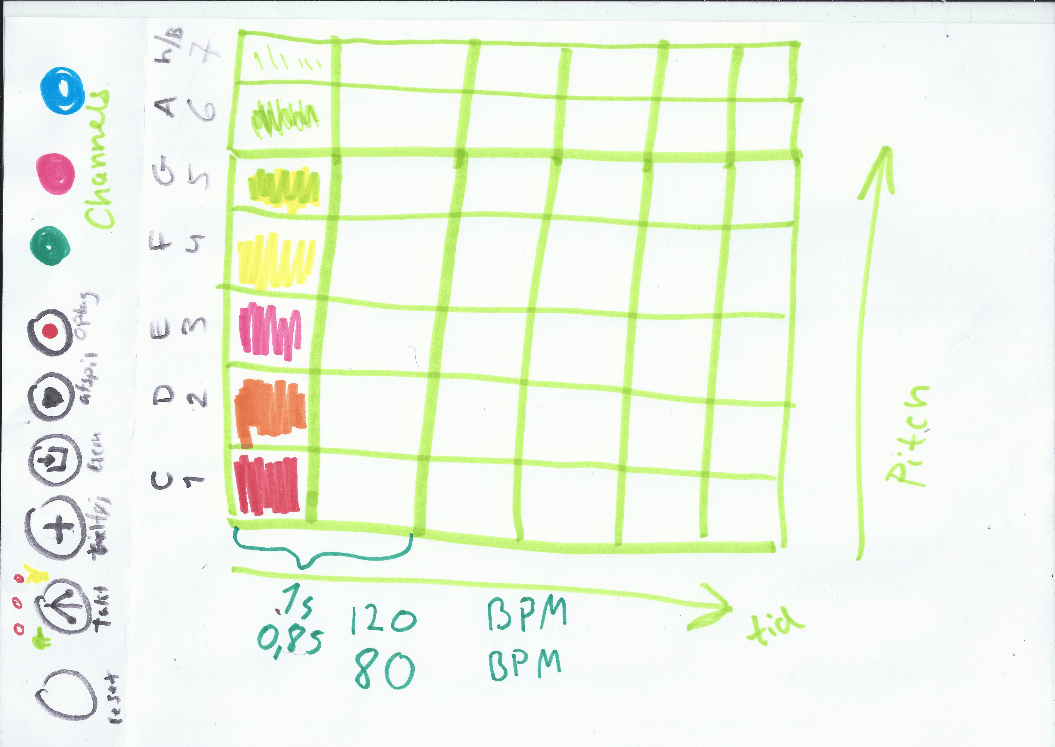
\includegraphics[width=0.9\linewidth]{figure/Design/firstSketchOfMat} 
	\caption{Seen is the first sketch of the interface for the sequencer-Mat concept . In the middle of the figure, is a green 7x6 grid - each field should activate a sound when stepped on. The horizontal axis of this grid, indicates time. The vertical axis indicates pitch of the sound. The pitch is also indicated by a color scheme along the same axis, variating from a dark to a light color. This is illustrated in the first column of the grid. Along same axis are the tone names stated besides their given rows. To the left of the grid are 9 push buttons (drawn as circles) with different functions (indicated with symbols and text) placed vertical. }
	\label{fig:firstSketchOfMatFig}
\end{figure}

To clarify how the basic sequencer functionality (play and record) should function, an example of a use case has been made. \\
\paragraph{Example of an use case}
Three students wants to play and record a set of tones which they want to consists of 3 tones with a break between each tone. They wants to play the tones F, C and G, respectively. The students place themselves on the mat, which the most left field activated (stepped on) being the tone F, then an empty column, then an activated field of the tone C, one more empty column, and lastly an activated field of the tone G. As so, it can be seen, that the tones are played from left to right.   
\begin{figure}[H]
	\centering
	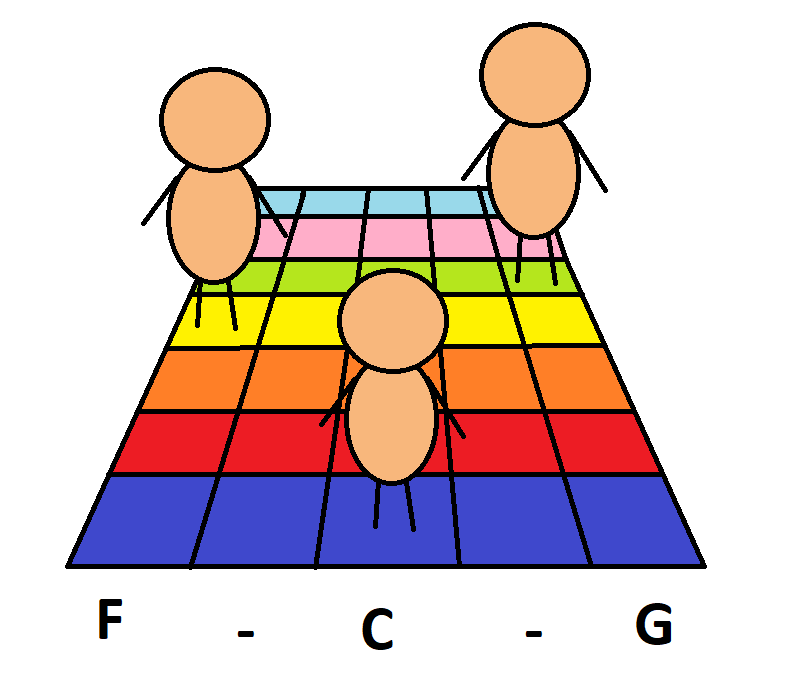
\includegraphics[width=0.7\linewidth]{figure/Design/UseCase} 
	\caption{Seen is an example of a use case of the sequencer mat tool. Three students are using the tool, recording the tones in the order of F, break, C, break, G. }
	\label{fig:UseCase2}
\end{figure}
  

To conclude on the two proposals, this (sequencer mat) concept included more of the desired elements gained from the workshop (\autoref{sec:workshop}), as well as having a more clear relation to the study plan (see \autoref{sec:studyPlan}) than the previous proposal,
it was therefore decided to continue working with this concept proposal (\autoref{sequencerMat}), as being the definitive design concept. 

\section{The Final design}\label{designConcept}
The concept, as explained in \autoref{sequencerMat}, was kept in the final design, however a lot of specification of functionalities and design was needed. These include the size, tempo, and musical scale of the mat, how the scale and time axis should be visualized, which functionalities (in form of buttons) should be implemented, where they should be placed, and how they should be visualized. 


\subsection{The setup}
The concept of the design includes visible functionality controls (buttons), and - without going far into implementation aspects of the design (is to be explained in \autoref{imp}), it was known that both these, and the mat itself, needed to be controlled by some electronics. For the sake of securing and protecting the electronic components, a box was chosen to become the housing of same, and as well, function as a interface for which the controls (buttons) should be placed. 

The placement of this control box in relation to the mat, was discussed, and it became clear, that the portability (so it could be transported for later testing), would have a high influence on the design. As it can be seen in \autoref{fig:matVsBox}, many different solutions were discussed. A suggestion was to have the box fasten along one side of the mat. Another was to have it fasten in continuation of the middle column of the mat grid, and maybe have the mat constructed to be collapsible. Lastly a suggestion was to make the mat and the box to be transported separately, and to be connected though a cable connector.     

\begin{figure}[H]
	\centering
	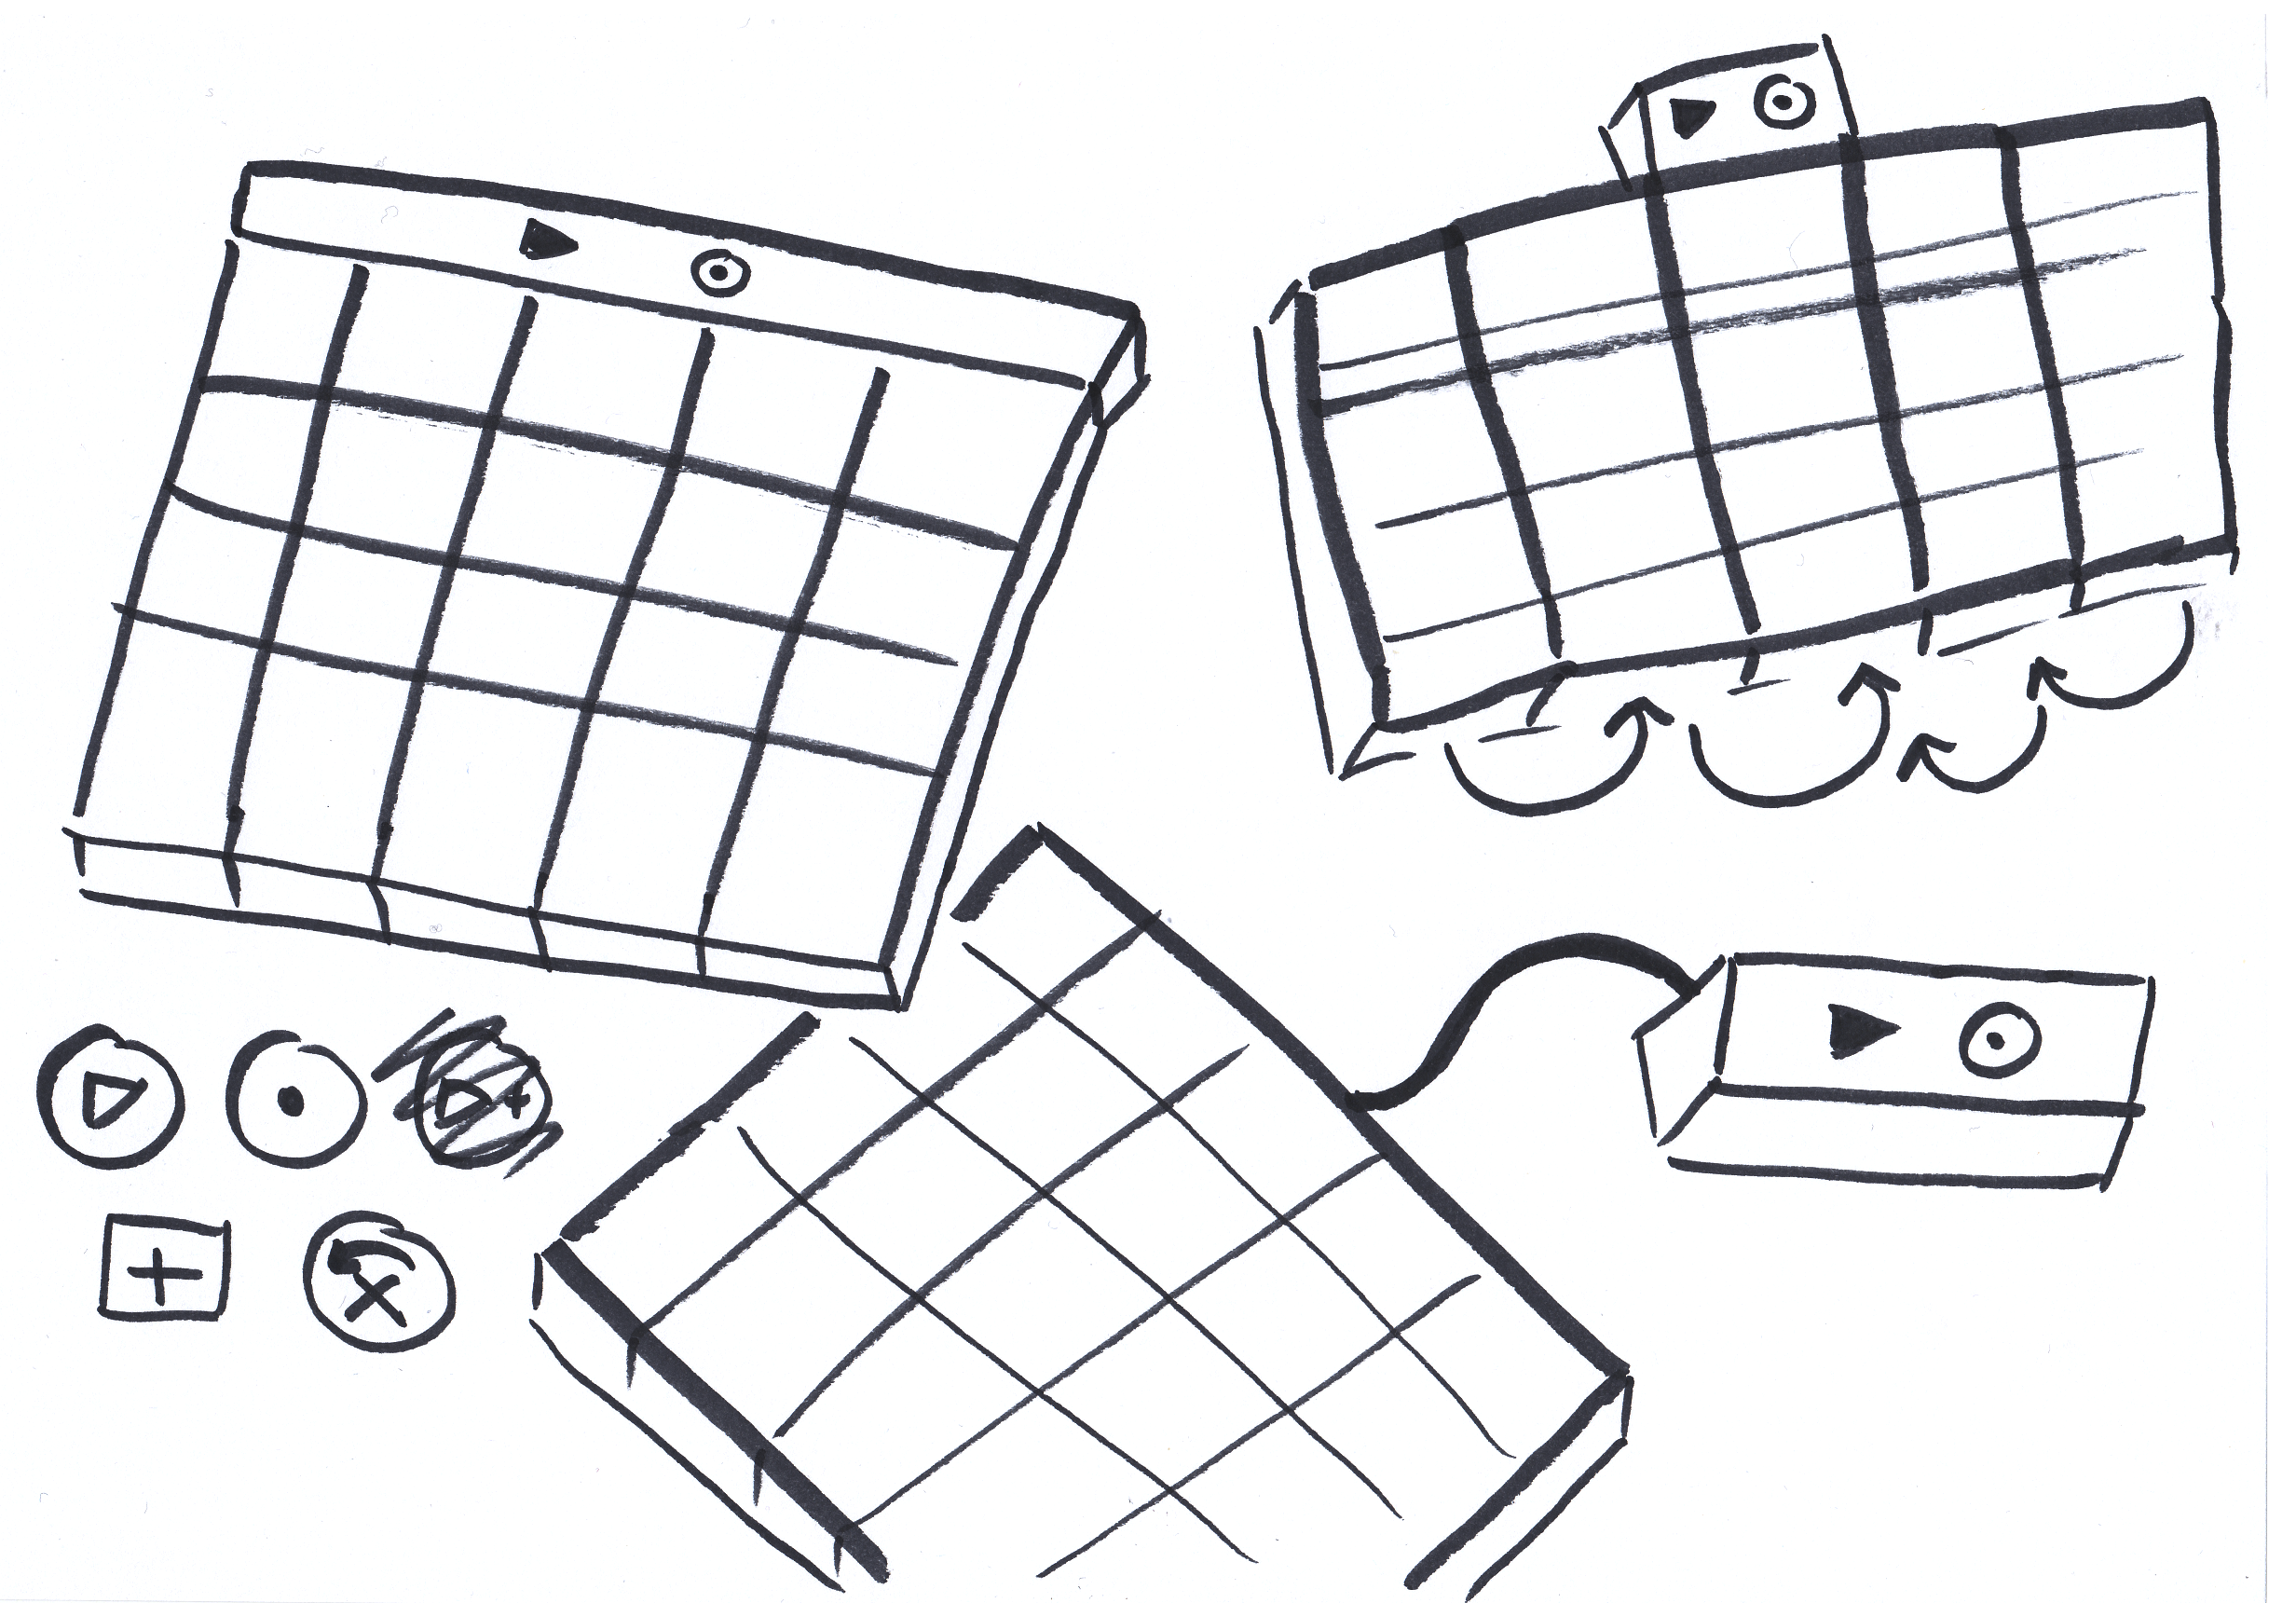
\includegraphics[width=0.7\linewidth]{figure/Design/maatteSetup}
	\caption{Seen is the different proposals to how the mat and box should be connected. Top left is the box fasten along the edge of the mat. Top right is the box fasten to the top of one column of the mat, which is collapsible. At the bottom is the box and mat connected though a detachable cable}
	\label{fig:matVsBox}
\end{figure} 

The material for construction the mat, was not yet chosen (Materials will be discussed in \autoref{theMat}), which made it uncertain if fasten the box(which was to be made of a hard material for protection of the electrical components), would be possible. For example if the mat was to be constructed by a flexible material, the connection joints between the mat and the box, might become overly exposed.
As the later of the suggestions, where the mat and box was to be manually connected though a cable, did not depend on the choice of material, this design was chosen. 


\subsection{The size and sound of the mat } \label{sizeSoundColorMat}
The size of the mat, effects the number of different tones it can produce, as the number of fields on the vertical axis is equivalent to the number of tones available. As this tool, should be used to create and perform music in an educational context (which relates to the study plan, see \autoref{studyPlan}), using a musical scale would be appropriate in relation to learning scales, and it would furthermore establish a hierarchy of the tones, due to the tonal context(which relates to the design principles\autoref{gestalt} of proximity and continuation) present in a scale \autoref{cognitiveFoundationOfPitch}, and thereby aid the student in understanding which field to stand on, to get the desired tone - making the tool more usable.  \\
Of the most common and primitive scales, are the major and minor scales (also called \textit{natural scales}), which consist of 7 notes (C D E F G A H/B - This is the C major scale) \cite{scales}. As one of these scales could have been chosen for this project, the \textit{Pentatonic scale}, which origins from the natural scales, have a few advantages for which it instead was chosen. The Pentatonic scale consist of five - hereof \textit{"penta"} - of the notes from the natural scale (C D E G A - this is the C major pentatonic scale), and has both the advantage of being able to be used in the same context as the natural scales, as well as sounding great no matter the combination of the notes \cite{pentatonicScale}. This makes this scale highly suitable for improvisational music, and beginners \cite{pentatonicScale}.  \\\\ 

With the pentatonic scale chosen for the tool, the vertical size of the mat was settled - 5 fields pr row. As the number of columns equivalents to the tempo of the sequencer function, and should therefore also reflect the musical aspect of tempo. A large variety of tempo could have been chosen, but as the most commonly used time is $\dfrac{4}{4} $ \cite{tempo}, this was decided as the rhythm of the tool. \\ As so, the size of the mat was decided to be 5x4 as seen on \autoref{fig:matSize}. As for the size of each field within the grid, the size of 27x27cm was chosen, based on the assumption that 4th graders have a shoesize ranging from size 35(EU) - 38(EU), which is approximately 22 - 25cm. This means that there will be room for one student pr field.       


\begin{figure}[H]
	\centering
	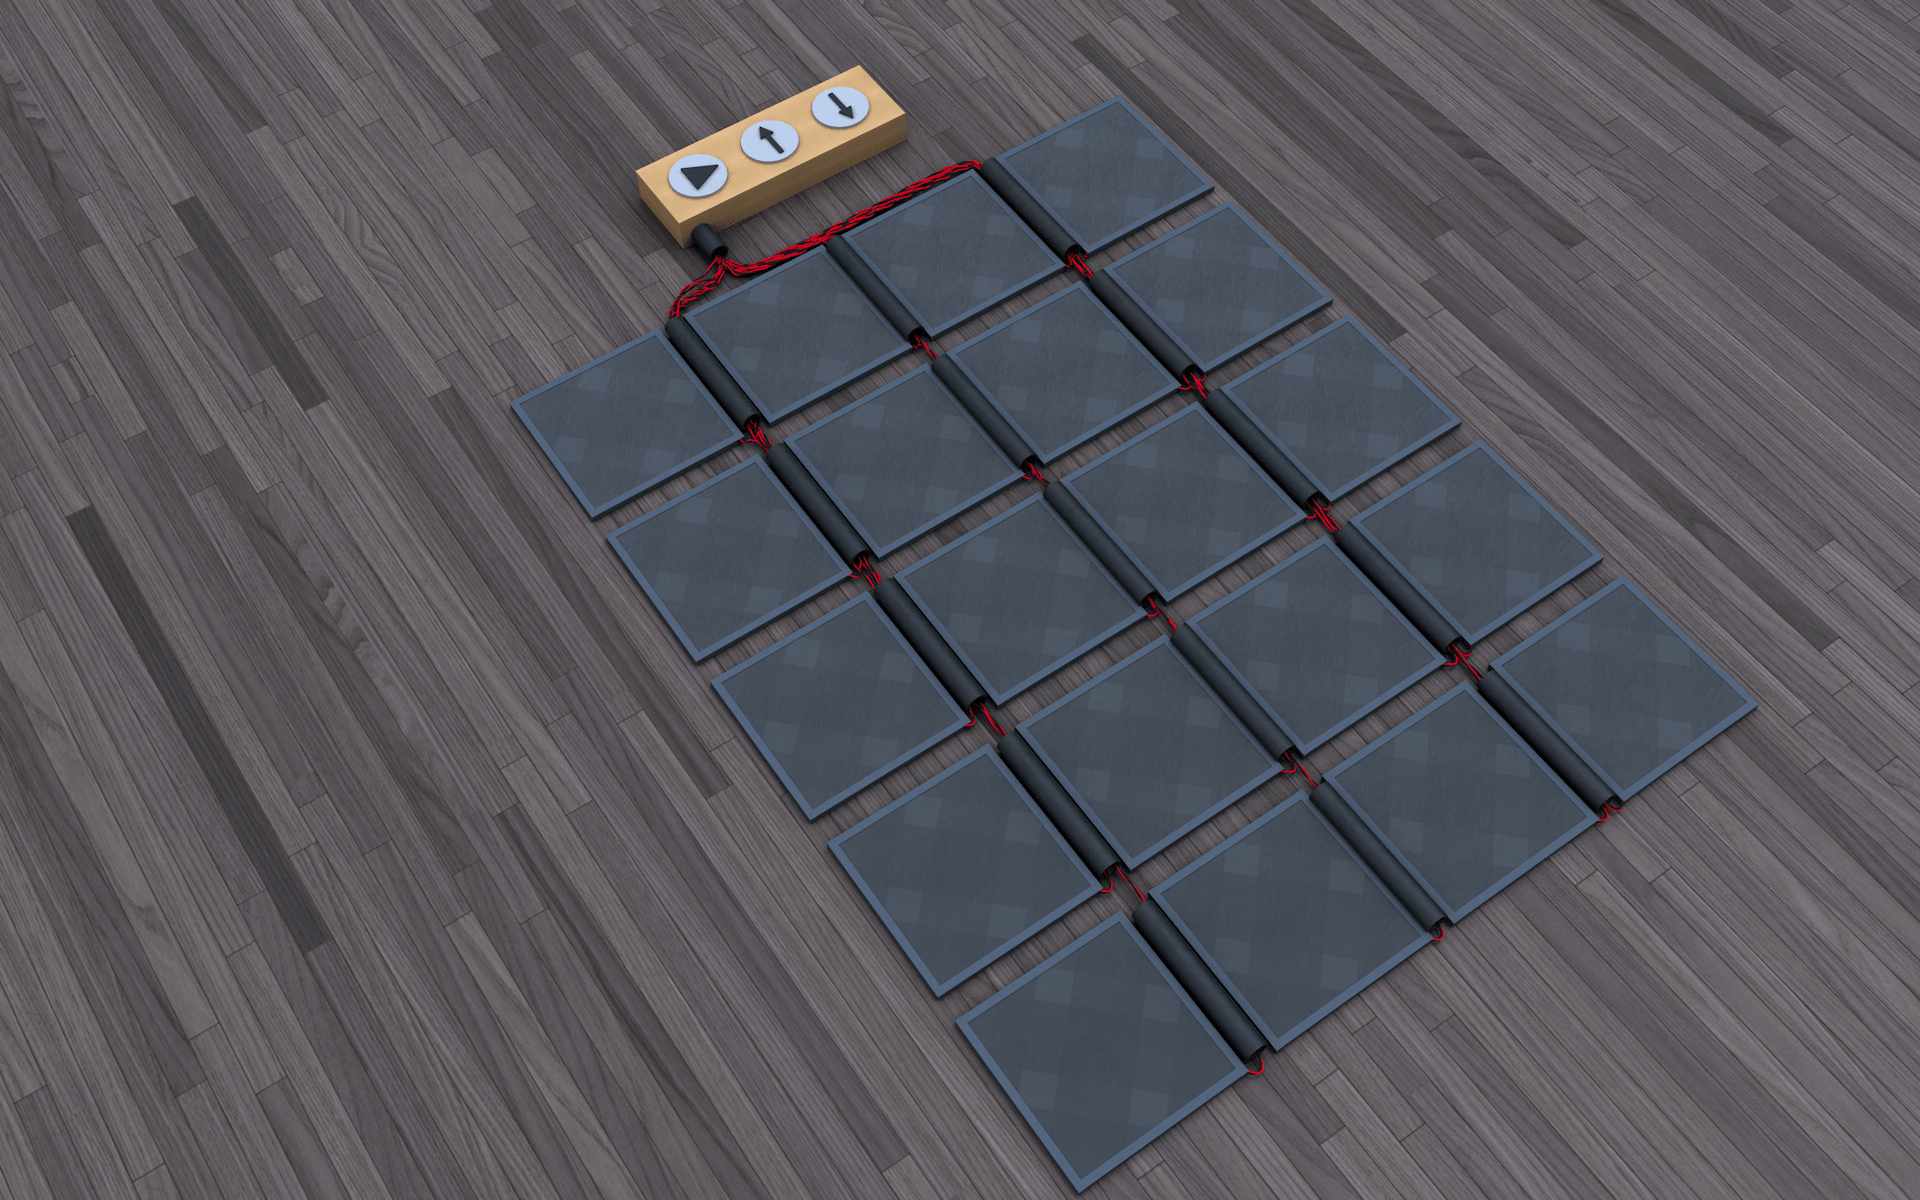
\includegraphics[width=0.8\linewidth]{figure/Design/finaldesign}
	\label{fig:matSize}
	\caption{Seen is a computer generated visualization of the size of the mat (a 5x4 grid), and the placement of the control box in relation to this.}
\end{figure}

To visualize the tonal context - ranging from a dark to a light tone, from bottom to top of the column - it was decided to use color to represent this transition. A color scheme was therefore to be chosen. Four out of five of the discussed color schemes can be seen on \autoref{colors} - missing is a gray scale gradient. The different color schemes discussed, was created with the intention of making a transition from a light to a dark color, resembling the tonal context. During the discussion, it became clear that the brightness of colors, was perceived different between individuals. For example could the green color be perceived brighter than the yellow by one person, while the opposite applied to another. To avoid confusion and ensure a common understanding for the transition, it was decided to use five different nuances/brightnesses of the same color. Two examples of this can be seen on \autoref{fig:colors}  - the two bottom ones. The orange color scheme was chosen, as this - in comparison to the blue, is often refereed to as a energetic color \cite{orange}, and was in relation to the physical active context of the tool, more suitable in the minds of the project group.               

\begin{figure}[H]
	\centering
	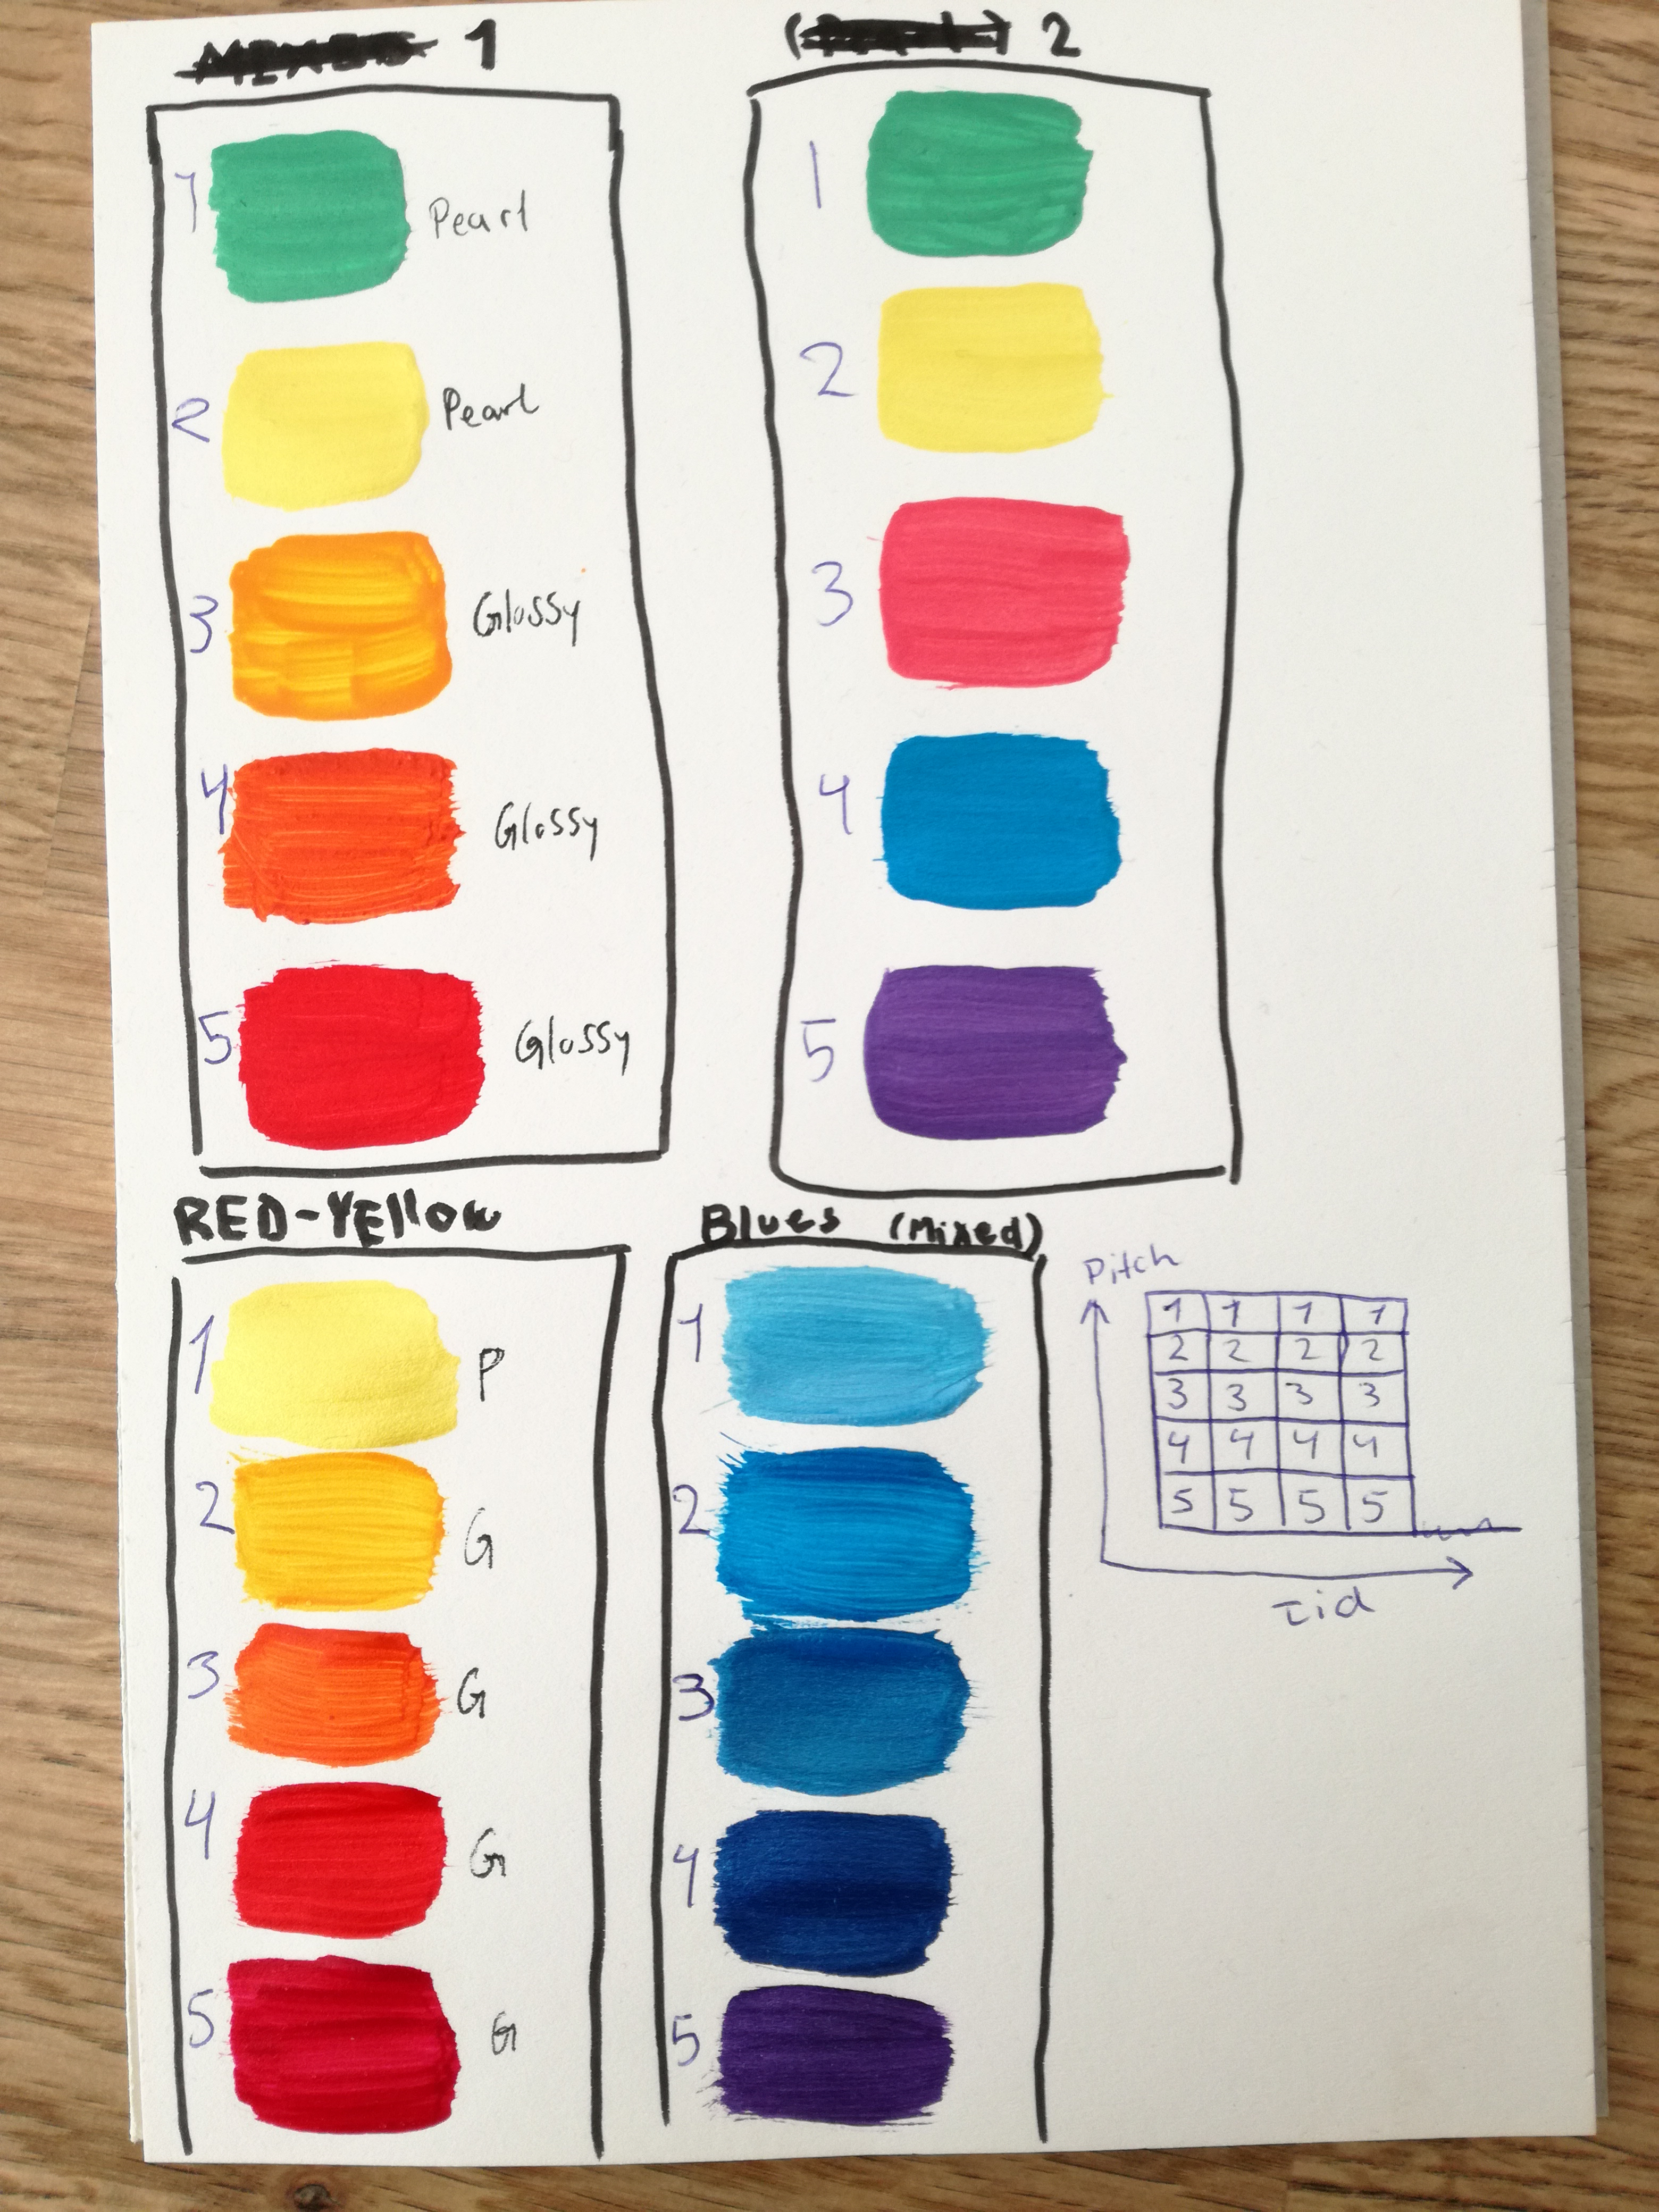
\includegraphics[width=0.5\linewidth]{figure/Design/colors}
	\caption{The four different color schemes (excluding a gray scale gradient), which was discussed for visualizing the tonal context.}	
	\label{fig:colors}
\end{figure}

To enhance the understanding of the columns as having the same tones, the design principle of similarity was used, by using the same color scheme for each column, as seen on \autoref{coloredMat}. \\
As so, by adding these decisions for colors and design principle, it should be visualized, that the fields with the same color, produce the same tone, and that each column contains one of each tone.  

\begin{figure}[H]
	\centering
	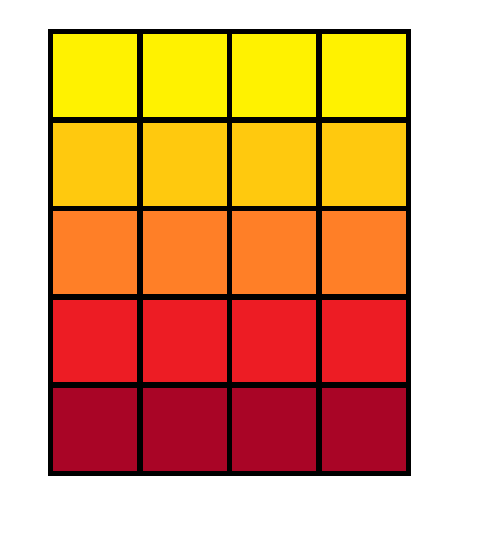
\includegraphics[width=0.5\linewidth]{figure/Design/coloredMat}
	\caption{Seen is a visualization of how the mat should be colored.}	
	\label{fig:coloredMat}
 \end{figure}


\subsection{The control box}
The control box functions, is as stated, both as protection for the hardware, as well as a interface for the controls of the sequencer. In this section, the thoughts concerning the dimensions of the box will be stated, and the functionalities for the sequencer and the visualizing of relating buttons, will be discussed.

\subsubsection{The dimensions} 
First of all, should the box be big enough to store the wires and components of the system. Besides this, the dimensions should take the use and possible misuse into consideration. With this is meant that actions such as using the controls on the box, should not make it fall over - it should be steady, and that jumping on the box (misuse) might be avoided by having a considerably large height of the box. The last mentioned, would also effect the extend to which the student will have to bend down to use the controls, maybe making it both more pleasant to use, and less tempting to try to use the controls with ones feet (misuse). The box should however remain a relatively small size, as it should be easily transportable. \\ 
All of this taking into consideration, the dimensions of the box was decided to be, around the size of a A4 paper for the interface side, and a height larger than the mats, but still small enough to give the box a low center of gravity to prevent it from falling over.

\subsubsection{The controls - function and visuals} 
The sequencer functions such as play, record etc., should be settled upon in order to establish the overall functionality of the tool, the numbers of controls(buttons) and their design. \\  The discussed functionalities, are:  

\begin{itemize}
	\item Play 
	\item Record 
	\item Delete
	\item Volume
	\item Octave up/down (this is to alter the tones pitch)
	\item sequences / "savepoints" (a number of entries to save on and play from)
	\item Channels/tracks (To play from multiple sequences at the same time)
	\item Save/add
	\item time/pace/metronome (to alter the tempo)
	\item reset
\end{itemize}   

As the tools main purpose for this project, is to facilitate collaboration, it was decided to minimize the number of functionalities to keep the complexion of the tool to a minimum. The functionalities chosen was therefore limited to \textit{play}, \textit{record}, \textit{delete} \textit{four sequences}, and \textit{octave up/down}. \textit{Play}, \textit{delete} and \textit{record}, are the most basic functionalities of, and defines a sequencer. \\
The sequences functionality, was chosen in order to let the uses make creations longer than four tones (which would be the case if there were only one sequence). The choice of having four sequences relates to the fact that music often builds upon even numbers, for which four is both one of the more common ones \cite{tempo}, and creates room enough for small melodies to be created. \\
The octave up/down was decided to be implemented even though it could be seen as an additional feature. This is due to the limited number of tones available when "only" having five different fields. By being able to change the octave of the tones, more tones will be available, and therefore enable the possibility to create and replicate melodies which spans over multiple octaves (example of a such song: \textit{"frere jacques"}).
\\\\
As it is know known which functions to implement, the control buttons for these can be designed.\\
The tree most bacis functionalities (play,delete,record) was solely based on the commonly used symbols for same functions (Used in for example \textit{Garage band} \cite{Garageband}). \\The sequences buttons was chosen to be visualized as numbers, as this might signify that the sequence of 1 should be recorded and played before sequence 2, and so forward. To indicate active sequences, an led for each should be lid if the related sequence is active. \\ The octave buttons was designed as arrows pointing in the up and down direction, to indicate the shift towards same. The button designs can be seen in a render of same, in \autoref{fig:buttonDesign}. \\ the placement of the buttons in relation to each other was settled upon using the gestalt principles \cite{gestalt} as guidance. The three main functionalities should be the same size of buttons (similarity\cite{gestalt}), and should be placed close together (proximity\cite{gestalt}).The sequence buttons should be smaller and placed together following the same principles. The LEDs related to the buttons, should also follow the principle of proximity, by being placed close to the buttons, as well as the relating pairs (button and LED) should be placed directly above/under each other - indicating that the given LED relates to the below sequence. \\ The octave buttons follow same principles as the the other groups of buttons - size similarity, and proximity.    
 

\begin{figure}[H]
	\centering
	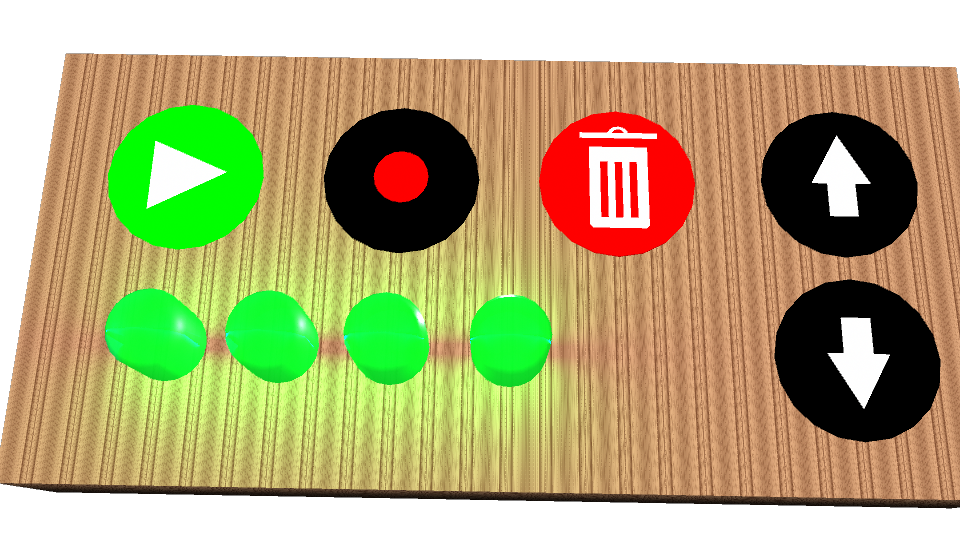
\includegraphics[width=0.7\linewidth]{figure/Design/buttonDesign}
	\label{fig:buttonDesign}
	\caption{Text goes here.}	
\end{figure}

\begin{figure}[H]
	\centering
	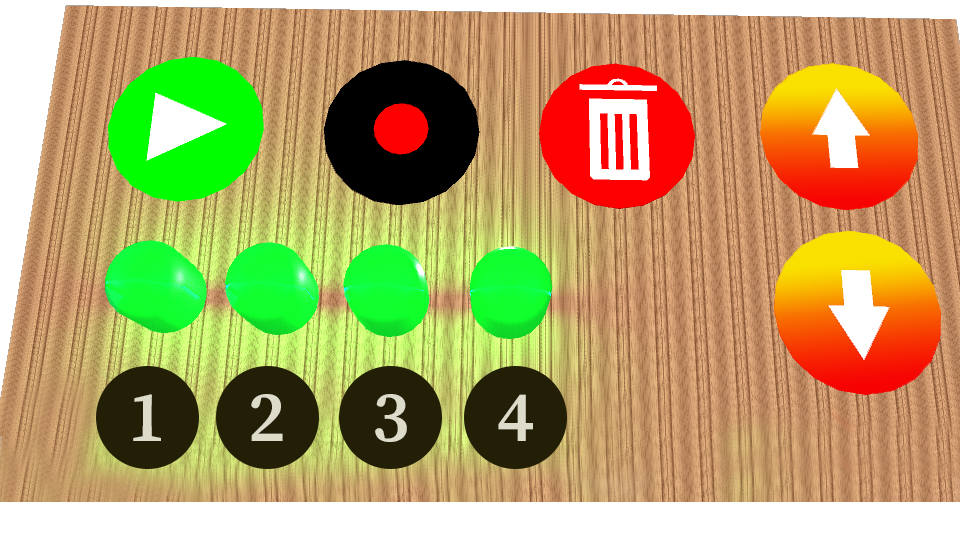
\includegraphics[width=0.7\linewidth]{figure/Design/buttonDesign2}
	\label{fig:buttonDesign2}
	\caption{Text goes here.}	
\end{figure}




By visualizing the tool with all of the design decisions made in this chapter, the final design should resemble \autoref{fig:designFinal}. The implementation of the mat will be described in the following chapter \autoref{imp}.  
\begin{figure}[H]
	\centering
	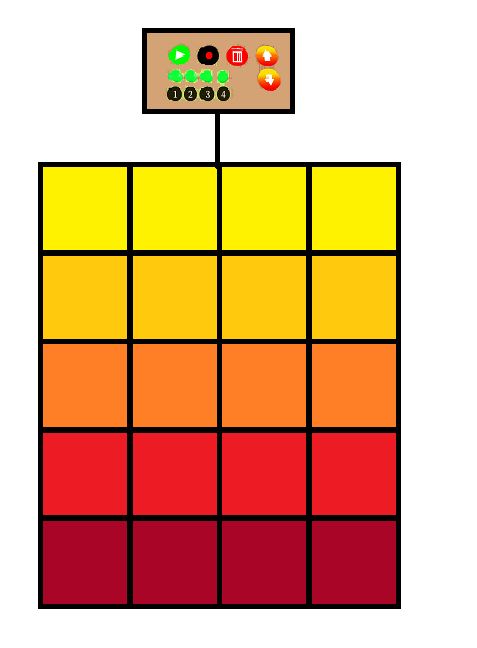
\includegraphics[width=0.7\linewidth]{figure/Design/DesignFinal}
	\label{fig:designFinal}
	\caption{A visualization of the final design.}	
\end{figure}













\section{Testing the design - Usability}
To test the usability of the mat and the control panel on the box a Usability test was conducted. This section explains how this test was prepared and executed. Furthermore, the findings from the test will be described.

\subsection{Preparations of test}
The goal of the test is to determine how usable the prototype is by the users and to eliminate possible challenges that might arise while interacting with the system. By having the test participants comp+-+lete a few tasks based on some of the use cases, that the prototype was designed for, and by observing how they manage to complete said tasks will indicate how the general usability of the system is and where the prototype is causing problems. To gather concrete data from the test the System Usability Scale(SUS)\cite{susScale} was used. It is a 10-item likert scale that is used to evaluate the usability of any given interactive system with both positively and negatively worded items. Based on prior research item 8 of the SUS-scale was reworded so the word \textit{cumbersome} was replaced by the word \textit{awkward}\cite{susScale}.


\subsection{Location}
The test participants for the usability test were found by convenience sampling around campus on Aalborg University Copenhagen (AAU CPH) as mentioned in \ref{chap:methods}. The participants were brought into a small room either as one person at a time or in pairs. The total number of participants was 10 (2 one-person tests and 4 pairs). The mat had been placed in the middle of the room and two computers were made available for the post test SUS-questionnaire. Furthermore, a moderator and two observers were present. In \autoref{fig:usabilityTest} the layout for the test is presented.

\begin{figure}[H]
	\centering
	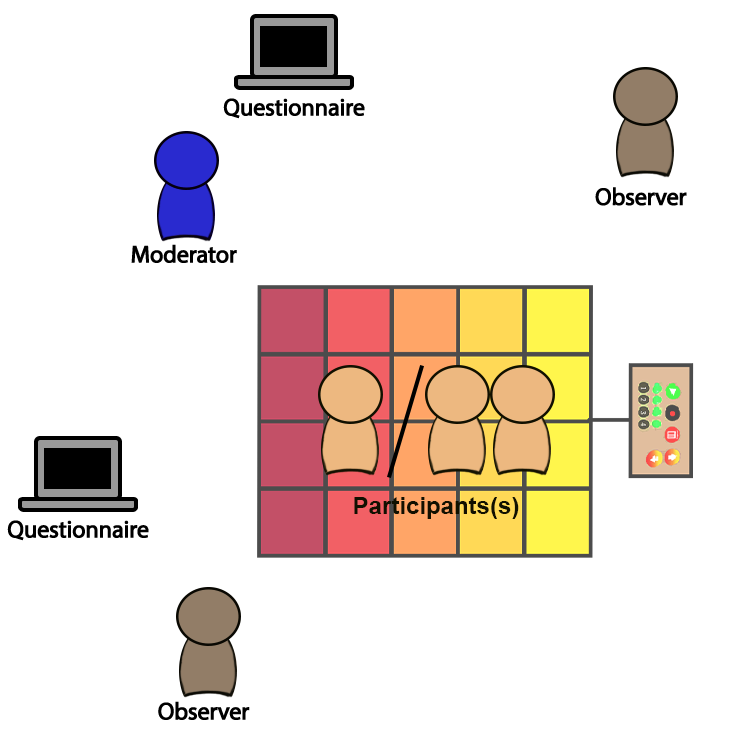
\includegraphics[width=0.7\linewidth]{figure/Design/usability}
	\caption{Figure showing the test layout during the Usability test.}	
	\label{fig:usabilityTest}
\end{figure}

\subsection{Test procedure and observations}

The participants were briefly introduced to the mat and the control panel and were then asked to explore the mat to get a feel of the layout. During this exploration most of the participants quickly discovered the correlation between the color scheme and the tones. They were then asked to change the octaves and this caused some problems. The octave buttons (arrows up and down) were confused with volume buttons and therefore a lot of the participants would try to push the Sequence buttons when asked to octavate. When discovering the octave buttons, sometimes with help from the moderator, the next task was completed with more ease as they were asked to lower the octave again. Afterwards, the participants were asked to record a short sequence and every time they would press the record button and then walk freely around on the mat and try to stop recording by pressing the record button again. When asked to play back what they recorded they would discover that the recording did not sound anything like what they played as the sequencer-like mechanism which makes the mat only record one column/beat at a time was not understood. Finally, they were asked to make sense of the control panel and explain in their own word, what they would expect the different buttons did. The icons on the play, record and delete buttons were self explanatory for most participants, however the sequence buttons were not. There was a lot of different explanations as to what the numbered buttons did e.g. add various filters and effects, change the scale, toggle buttons for enabling/disabling the columns of the mat as the number of columns and the number of sequences were the same. When all the tasks were completed some participants would comment on the lack of indication of which column/beat was playing when they recording. Also, they requested indicators on the control panel to make it more clear what the buttons did. After the test the participants were asked to fill out a SUS-questionnaire on one of the two available computers which was the final part of the usability test.

\subsection{SUS Questionnaire}
In \autoref{fig:susResults} the results from the SUS-questionnaire, that followed the Usability test, are visualized in the form of a box plot graph. The following is a list of the questions from the SUS scale. The odd-numbered items in blue are considered the positively worded questions, whereas the even-numbered i-+tems in red are worded negatively. This is relevant for later analysis of the results.\\

\begin{enumerate}
	\item  \textcolor{blue}{I think that I would like to use this system frequently.}
	\item  \textcolor{red}{I found the system unnecessarily complex.}
	\item  \textcolor{blue}{I thought the system was easy to use.}
	\item  \textcolor{red}{I think that I would need the support of a technical person to be able to use this system.}
	\item  \textcolor{blue}{I found the various functions in this system were well integrated.}
	\item  \textcolor{red}{I thought there was too much inconsistency in this system.}
	\item  \textcolor{blue}{I would imagine that most people would learn to use this system very quickly.}
	\item  \textcolor{red}{I found the system very awkward to use.}
	\item  \textcolor{blue}{I felt very confident using the system.}
	\item  \textcolor{red}{I needed to learn a lot of things before I could get going with this system.}
\end{enumerate} 
%SUS boxplot

\begin{figure}[H]
	\centering
	% This file was created by matlab2tikz.
%
%The latest updates can be retrieved from
%  http://www.mathworks.com/matlabcentral/fileexchange/22022-matlab2tikz-matlab2tikz
%where you can also make suggestions and rate matlab2tikz.
%
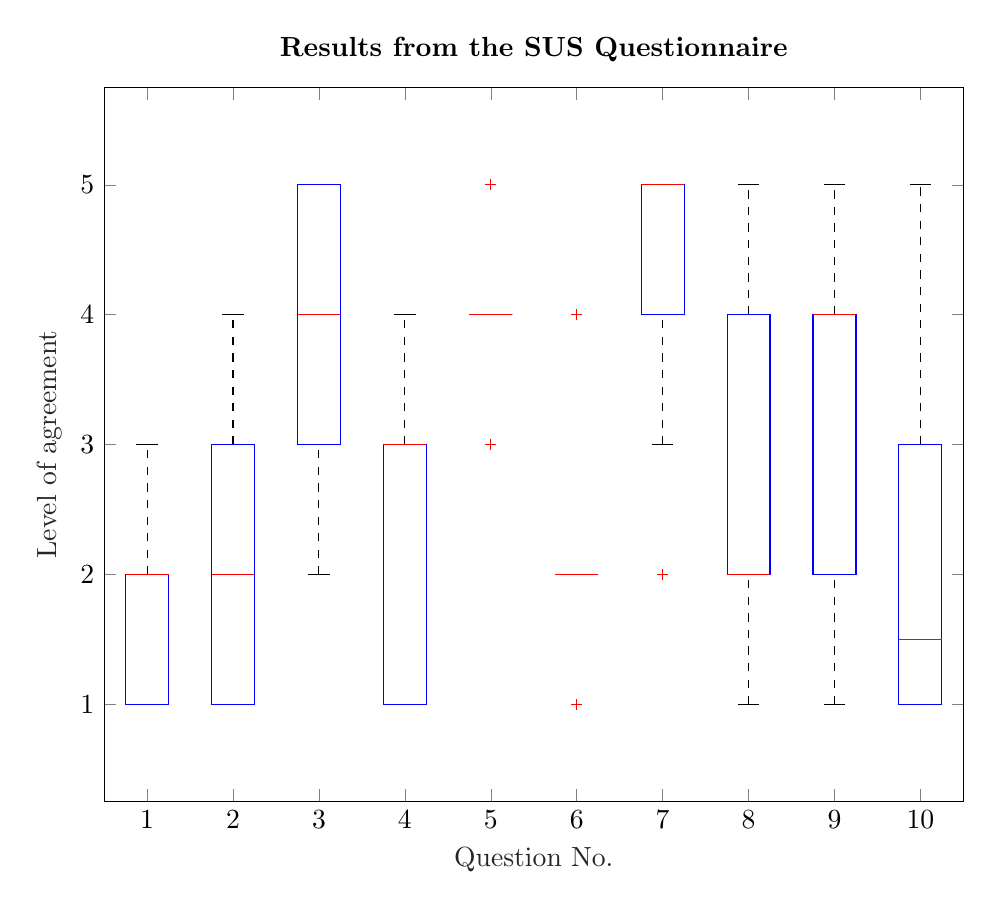
\begin{tikzpicture}

\begin{axis}[%
width=0.9\linewidth,
height=3.566in,
scale only axis,
unbounded coords=jump,
xmin=0.5,
xmax=10.5,
xtick={1,2,3,4,5,6,7,8,9,10},
xlabel style={font=\color{white!15!black}},
xlabel={Question No.},
ymin=0.257573175810164,
ymax=5.7459492315434,
ylabel style={font=\color{white!15!black}},
ylabel={Level of agreement},
axis background/.style={fill=white},
title style={font=\bfseries},
title={Results from the SUS Questionnaire},
legend style={legend cell align=left, align=left, draw=white!15!black}
]
\addplot [color=black, dashed, forget plot]
  table[row sep=crcr]{%
1	2\\
1	3\\
};
\addplot [color=black, dashed, forget plot]
  table[row sep=crcr]{%
2	3\\
2	4\\
};
\addplot [color=black, dashed, forget plot]
  table[row sep=crcr]{%
3	5\\
3	5\\
};
\addplot [color=black, dashed, forget plot]
  table[row sep=crcr]{%
4	3\\
4	4\\
};
\addplot [color=black, dashed, forget plot]
  table[row sep=crcr]{%
5	4\\
5	4\\
};
\addplot [color=black, dashed, forget plot]
  table[row sep=crcr]{%
6	2\\
6	2\\
};
\addplot [color=black, dashed, forget plot]
  table[row sep=crcr]{%
7	5\\
7	5\\
};
\addplot [color=black, dashed, forget plot]
  table[row sep=crcr]{%
8	4\\
8	5\\
};
\addplot [color=black, dashed, forget plot]
  table[row sep=crcr]{%
9	4\\
9	5\\
};
\addplot [color=black, dashed, forget plot]
  table[row sep=crcr]{%
10	3\\
10	5\\
};
\addplot [color=black, dashed, forget plot]
  table[row sep=crcr]{%
1	1\\
1	1\\
};
\addplot [color=black, dashed, forget plot]
  table[row sep=crcr]{%
2	1\\
2	1\\
};
\addplot [color=black, dashed, forget plot]
  table[row sep=crcr]{%
3	2\\
3	3\\
};
\addplot [color=black, dashed, forget plot]
  table[row sep=crcr]{%
4	1\\
4	1\\
};
\addplot [color=black, dashed, forget plot]
  table[row sep=crcr]{%
5	4\\
5	4\\
};
\addplot [color=black, dashed, forget plot]
  table[row sep=crcr]{%
6	2\\
6	2\\
};
\addplot [color=black, dashed, forget plot]
  table[row sep=crcr]{%
7	3\\
7	4\\
};
\addplot [color=black, dashed, forget plot]
  table[row sep=crcr]{%
8	1\\
8	2\\
};
\addplot [color=black, dashed, forget plot]
  table[row sep=crcr]{%
9	1\\
9	2\\
};
\addplot [color=black, dashed, forget plot]
  table[row sep=crcr]{%
10	1\\
10	1\\
};
\addplot [color=black, forget plot]
  table[row sep=crcr]{%
0.875	3\\
1.125	3\\
};
\addplot [color=black, forget plot]
  table[row sep=crcr]{%
1.875	4\\
2.125	4\\
};
\addplot [color=black, forget plot]
  table[row sep=crcr]{%
2.875	5\\
3.125	5\\
};
\addplot [color=black, forget plot]
  table[row sep=crcr]{%
3.875	4\\
4.125	4\\
};
\addplot [color=black, forget plot]
  table[row sep=crcr]{%
4.875	4\\
5.125	4\\
};
\addplot [color=black, forget plot]
  table[row sep=crcr]{%
5.875	2\\
6.125	2\\
};
\addplot [color=black, forget plot]
  table[row sep=crcr]{%
6.875	5\\
7.125	5\\
};
\addplot [color=black, forget plot]
  table[row sep=crcr]{%
7.875	5\\
8.125	5\\
};
\addplot [color=black, forget plot]
  table[row sep=crcr]{%
8.875	5\\
9.125	5\\
};
\addplot [color=black, forget plot]
  table[row sep=crcr]{%
9.875	5\\
10.125	5\\
};
\addplot [color=black, forget plot]
  table[row sep=crcr]{%
0.875	1\\
1.125	1\\
};
\addplot [color=black, forget plot]
  table[row sep=crcr]{%
1.875	1\\
2.125	1\\
};
\addplot [color=black, forget plot]
  table[row sep=crcr]{%
2.875	2\\
3.125	2\\
};
\addplot [color=black, forget plot]
  table[row sep=crcr]{%
3.875	1\\
4.125	1\\
};
\addplot [color=black, forget plot]
  table[row sep=crcr]{%
4.875	4\\
5.125	4\\
};
\addplot [color=black, forget plot]
  table[row sep=crcr]{%
5.875	2\\
6.125	2\\
};
\addplot [color=black, forget plot]
  table[row sep=crcr]{%
6.875	3\\
7.125	3\\
};
\addplot [color=black, forget plot]
  table[row sep=crcr]{%
7.875	1\\
8.125	1\\
};
\addplot [color=black, forget plot]
  table[row sep=crcr]{%
8.875	1\\
9.125	1\\
};
\addplot [color=black, forget plot]
  table[row sep=crcr]{%
9.875	1\\
10.125	1\\
};
\addplot [color=blue, forget plot]
  table[row sep=crcr]{%
0.75	1\\
0.75	2\\
1.25	2\\
1.25	1\\
0.75	1\\
};
\addplot [color=blue, forget plot]
  table[row sep=crcr]{%
1.75	1\\
1.75	3\\
2.25	3\\
2.25	1\\
1.75	1\\
};
\addplot [color=blue, forget plot]
  table[row sep=crcr]{%
2.75	3\\
2.75	5\\
3.25	5\\
3.25	3\\
2.75	3\\
};
\addplot [color=blue, forget plot]
  table[row sep=crcr]{%
3.75	1\\
3.75	3\\
4.25	3\\
4.25	1\\
3.75	1\\
};
\addplot [color=blue, forget plot]
  table[row sep=crcr]{%
4.75	4\\
4.75	4\\
5.25	4\\
5.25	4\\
4.75	4\\
};
\addplot [color=blue, forget plot]
  table[row sep=crcr]{%
5.75	2\\
5.75	2\\
6.25	2\\
6.25	2\\
5.75	2\\
};
\addplot [color=blue, forget plot]
  table[row sep=crcr]{%
6.75	4\\
6.75	5\\
7.25	5\\
7.25	4\\
6.75	4\\
};
\addplot [color=blue, forget plot]
  table[row sep=crcr]{%
7.75	2\\
7.75	4\\
8.25	4\\
8.25	2\\
7.75	2\\
};
\addplot [color=blue, forget plot]
  table[row sep=crcr]{%
8.75	2\\
8.75	4\\
9.25	4\\
9.25	2\\
8.75	2\\
};
\addplot [color=blue, forget plot]
  table[row sep=crcr]{%
9.75	1\\
9.75	3\\
10.25	3\\
10.25	1\\
9.75	1\\
};
\addplot [color=red, forget plot]
  table[row sep=crcr]{%
0.75	2\\
1.25	2\\
};
\addplot [color=red, forget plot]
  table[row sep=crcr]{%
1.75	2\\
2.25	2\\
};
\addplot [color=red, forget plot]
  table[row sep=crcr]{%
2.75	4\\
3.25	4\\
};
\addplot [color=red, forget plot]
  table[row sep=crcr]{%
3.75	3\\
4.25	3\\
};
\addplot [color=red, forget plot]
  table[row sep=crcr]{%
4.75	4\\
5.25	4\\
};
\addplot [color=red, forget plot]
  table[row sep=crcr]{%
5.75	2\\
6.25	2\\
};
\addplot [color=red, forget plot]
  table[row sep=crcr]{%
6.75	5\\
7.25	5\\
};
\addplot [color=red, forget plot]
  table[row sep=crcr]{%
7.75	2\\
8.25	2\\
};
\addplot [color=red, forget plot]
  table[row sep=crcr]{%
8.75	4\\
9.25	4\\
};
\addplot [color=red, forget plot]
  table[row sep=crcr]{%
9.75	1.5\\
10.25	1.5\\
};
\addplot [color=black, draw=none, mark=+, mark options={solid, red}, forget plot]
  table[row sep=crcr]{%
nan	nan\\
};
\addplot [color=black, draw=none, mark=+, mark options={solid, red}, forget plot]
  table[row sep=crcr]{%
nan	nan\\
};
\addplot [color=black, draw=none, mark=+, mark options={solid, red}, forget plot]
  table[row sep=crcr]{%
nan	nan\\
};
\addplot [color=black, draw=none, mark=+, mark options={solid, red}, forget plot]
  table[row sep=crcr]{%
nan	nan\\
};
\addplot [color=black, draw=none, mark=+, mark options={solid, red}, forget plot]
  table[row sep=crcr]{%
5	3\\
5	3\\
5	5\\
5	5\\
};
\addplot [color=black, draw=none, mark=+, mark options={solid, red}, forget plot]
  table[row sep=crcr]{%
6	1\\
6	1\\
6	4\\
6	4\\
};
\addplot [color=black, draw=none, mark=+, mark options={solid, red}, forget plot]
  table[row sep=crcr]{%
7	2\\
};
\addplot [color=black, draw=none, mark=+, mark options={solid, red}, forget plot]
  table[row sep=crcr]{%
nan	nan\\
};
\addplot [color=black, draw=none, mark=+, mark options={solid, red}, forget plot]
  table[row sep=crcr]{%
nan	nan\\
};
\addplot [color=black, draw=none, mark=+, mark options={solid, red}, forget plot]
  table[row sep=crcr]{%
nan	nan\\
};
\end{axis}
\end{tikzpicture}%
	\caption{Figure showing the results of the SUS-questionnaire. The question numbers on the x-axis correspond to the question numbers in the above list of SUS-items}	
	\label{fig:susResults}
\end{figure}

Due to the way the SUS-scale is constructed it is expected that the boxplots will alternate between high to low every other question in \autoref{fig:susResults} if the usability is sufficient. In this case we see that the first question is low even though it should be high. This particular question was \textit{I think that I would like to use this system frequently} and since the test participants were made aware of the actual target group as being elementary school children learning music the outcome of the first question is not surprising. Question 8, which was reworded to \textit{I found the system very awkward to use}, did not seem to cause any noticeable confusion as the participants filled out their questionnaire. However, results shows that there were mixed feelings towards the mat usage. This might be due to the fact that some of the pads on the mat started to behave more and more inconsistent throughout the day of the test.

\subsection{Findings}
To find out how the system scores on the SUS scale some calculation must be made. The scoring system of the SUS ranges from 0-100 with 2.5 increments. The calculation is shown below in \autoref{eq:susCalc}:

\begin{equation} \label{eq:susCalc}
( (Q_1+Q_3+Q_5+Q_7+Q_9)-5+25-(Q_2+Q_4+Q_6+Q_8+Q_{10}) )*2.5
\end{equation}
\linebreak
To calculate the score 1 point must be subtracted by each odd-numbered item and the even-numbered questions must be subtracted from 5. This is then multiplied by 2.5 to get the final score. \autoref{tab:susScoreTable} shows the calculated scores for each participant and the overall mean of the SUS scores for all tests.

\begin{table}[H]
	\centering
	\caption{Table showing the SUS score for each individual test participants and the overall mean score. For full table see appendix \ref{appendix:susResults}}
	\label{tab:susScoreTable}
	\begin{tabular}{|c|c|l|l|}
		\hline
		Participant & SUS Score \\ \hline
		1           & 52.5      \\ \hline
		2           & 75.0      \\ \hline
		3           & 45.0      \\ \hline
		4           & 55.0      \\ \hline
		5           & 75.0      \\ \hline
		6           & 37.5      \\ \hline
		7           & 70.0      \\ \hline
		8           & 80.0      \\ \hline
		9           & 70.0      \\ \hline
		10          & 75.0      \\ \hline
		Total       & 63.5      \\ \hline
	\end{tabular}
\end{table}

\autoref{fig:susScore} shows how the overall test score for the Usability test performs on the full scale from 0-100. As seen in the figure the total score is somewhere in between \textit{OK} and \textit{GOOD}, which means that there is some room for improvement.

\begin{figure}[H]
	\centering
	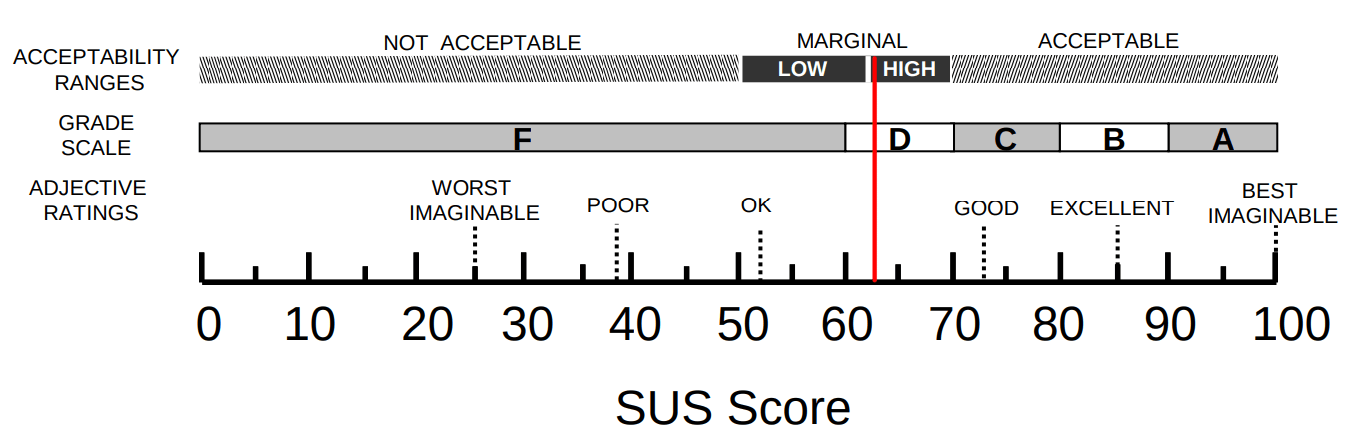
\includegraphics[width=1\linewidth]{figure/Design/susScore}
	\caption{Figure highlighting the test score(63.5) on a scale representing SUS scores and their meanings\cite{susScore}}
	\label{fig:susScore}
\end{figure}

\subsection{Summary}
As seen in \autoref{fig:susScore} the mat has some problems that should be fixed. The technical mat related issues are immediately apparent. Based on the observations and comments the two major problems were the missing button labels and beat indicators.

\section{Improvements to the final design}
 %  LED og klistermærker 
\todo{kan først skrives når usability er færdig da der skal refereres meget dertil :) }
